\documentclass[letterpaper]{article}

\usepackage{graphicx}
\usepackage{hyperref}
\usepackage[margin=1in]{geometry}
\usepackage{listings}
\graphicspath{ {./} }

\begin{document}

% Title -----------------------------------------------------------------------

\title{Reading 04: Diversity At Notre Dame}
\date{February 15, 2017}
\author{Jeff Klouda {\textless}jklouda1@nd.edu{\textgreater}}

\maketitle

% Overview --------------------------------------------------------------------

\section*{Overview}

\paragraph{
I used shell scripts and Gnuplots to analyze the gender and ethnicity data
of the students in Notre Dame's Computer Science program.  Plotting this data
from the classes of 2013 through 2019 as provided by Ramzi Bualuan of the 
Computer Science department, I was able to identify norms and trends in
diversity in the program.  The program has increased in size every year since
2014, and the students in the progrma have been and are largely Caucasian and
male.  While there have generally been more female students each year than in
the previous, they are still outnumbered by their male peers nearly two to
one, and while there has been a slight increase in the number of 
non-Caucasian students, there are still far more Caucasian students in the
program than students of other ethnicities.
}

% Methodology -----------------------------------------------------------------

\section*{Methodology}

\paragraph{
To process the demographics.csv data I used the two shell scripts 
printed below, gender.sh and ethnic.sh, that function similarly.  Each script
relies on a function that takes two input arguments; the count\_gender 
function in gender.sh takes the year and the gender to be totaled.  With 
these, it sets the column to search based on the year because the data in the
provided .csv if organized in columns by year.  It then uses the gender 
argument to determine what character to count in that column.  These 
variables are then used in the pipeline at the end of the function.  curl 
downloads the data from the specified URL, cut takes the specified column 
based on the comma delimiter, grep finds all lines in that column matching 
the specified gender, and wc -l lists the number of lines in that output, 
counting the number of matches.  This outputs the number of students of the 
specified gender in the specified year.  This pipeline runs in the for loop 
at the bottom of the script, calculating the number of students of each 
gender in each year present in the data and using echo to output this data in
the form of (year) (number of female students) (number of male students).  ethnic.sh 
functions in exactly the same way, but instead of taking gender as the 
second argument of its count\_ethnic function, it takes ethnicity as
represented by the characters C, O, S, B, N, T, and U.  The function uses
these characters in a pipeline identical to that used in the gender.sh script
to generate totals for students of each ethnicity in each year.  This 
function is run in the for loop at the bottom of the script for each
ethnicity each year, producing output in the for of the year followed by 
the number of students of each ethnicity in the data.}
\paragraph{
To produce the graphs in Figures \ref{fig:gender} and \ref{fig:ethnic}, I first
ran the gender.sh and ethnic.sh scripts to store the information from the 
demographics csv in tables in gender.dat and ethnic.dat.  This data can be 
seen in Tables \ref{tbl:gender} and \ref{tbl:ethnic}.  I then used these .dat
files and the provided .plt files and Makefile to plot the demographics data
in the gender.png and ethnic.png files.}
\paragraph{
I did not have too much difficulty extracting data or plotting it 
because of how much of the necessary code was provided in the Reading04 
assignment.  One aspect that I did struggle with was writing the arithmetic
expression to determine the column based on the year.  I was trying to use
the expr command, but it was not compatible with the way in which I was
formatting my expression.  I was able to use the arithmetic expression
\$(( )) notation instead to solve this problem.}


\pagebreak
% Code Listings


\lstinputlisting{gender.sh}
\vfill
\lstinputlisting{ethnic.sh}

% Analysis --------------------------------------------------------------------

\section*{Analysis}

\begin{enumerate}

\item{Overall, the data shows a trend toward a more balanced gender
distribution in the Computer Science and Engineering program.  As can 
be seen in Table \ref{tbl:gender} and Figure \ref{fig:gender}, there
have consistently been more students in general and more female
students in particular in the program.  This suggests that the program 
does seem to be moving toward a better gender balance despite the 
population of male students still greatly outnumbering that of female
students.}

\item{Ethnic diversity, as seen in Table \ref{tbl:ethnic} and Figure
\ref{fig:gender}, does not seem to have as significant an upward trend in the program as gender balance does.  The number of students of each ethnicity other than Caucasian seems fluctuate each year rather than trending one way or the other.  Caucasian students make up the vast majority of students in each year, and that does not seem to be changing.}

\end{enumerate}




% Discussion ------------------------------------------------------------------

\section*{Discussion}

\paragraph{}

\begin{enumerate}

\item{I think both this department and the technology industry in general should work to improve diversity.  Considering how prevalent the modern technology industry seems to be, there is no reason the people working in the industry should not be more representative of the population at large.  If the industry is to design effective solutions to be used by people of all genders and ethnicities, then these solutions need to be designed by people of all genders and ethnicities.  I think there is also something to the idea that people of different backgrounds approach problems differently and that by working in more diverse teams we are able to create better solutions.  This department should work to increase diversity in order to be more welcoming to students of underrepresented backgrounds and prepare students to bring more diversity to industry}

\item{I think the Computer Science and Engineering department does provide a largely welcoming and supporting environment.  All of the faculty I have interacted with have been supportive and friendly, and as someone with no previous experience in the field, I think the introductory courses have been well structured for newcomers.  I think maybe smaller class sizes and more group projects in the beginning classes would help to create a stronger community, but other than that, the atmosphere in the department has definitely been welcoming and supportive in my opinion.}

\item{I have not personally experienced any significant challenges in regards to diversity in the Computer Science and Engineering program.  I think the faculty has done an excellent job in supporting me and my peers thus far in our education.}

\end{enumerate}

\begin{table}[h]
    \centering
        \begin{tabular}{|c|c|c|}
            Year & Female & Male\\
            \hline
            2013 & 14 & 49\\
            2014 & 12 & 44\\
            2015 & 16 & 58\\
            2016 & 19 & 60\\
            2017 & 26 & 65\\
            2018 & 36 & 90\\
            2019 & 51 & 97\\
        \end{tabular}
    \caption{CSE Student Gender per Year}
    \label{tbl:gender}
\end{table}

\begin{table}[h]
    \centering
        \begin{tabular}{|c|c|c|c|c|c|c|c|}
            Year & Caucasian & Asian & Hispanic & African American & Native American
            & Multiple Selection & Undeclared\\
            \hline
            2013 & 43 & 7 & 7 & 3 & 1 & 2 & 0\\
            2014 & 43 & 5 & 4 & 2 & 1 & 1 & 0\\
            2015 & 47 & 9 & 10 & 4 & 1 & 1 & 2\\
            2016 & 53 & 9 & 9 & 1 & 7 & 0 & 0\\
            2017 & 60 & 12 & 3 & 5 & 5 & 6 & 0\\
            2018 & 91 & 8 & 12 & 3 & 4 & 8 & 0\\
            2019 & 92 & 13 & 10 & 3 & 15 & 14 & 0\\
        \end{tabular}
    \caption{CSE Student Ethnicity per Year}
    \label{tbl:ethnic}
\end{table}

\begin{figure}[h]
\centering
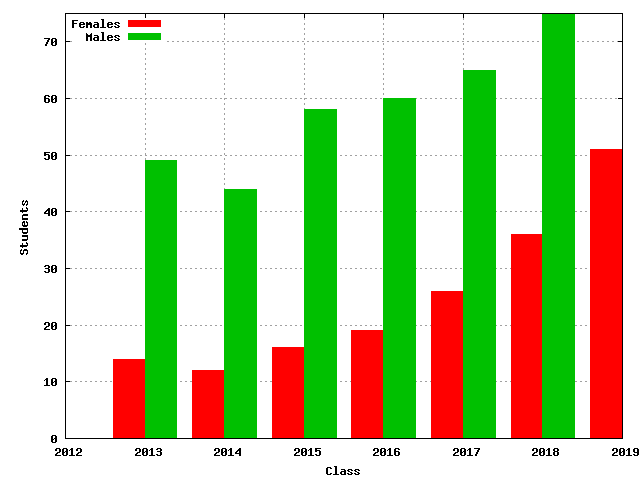
\includegraphics[scale=0.5]{gender.png}
\caption{CSE Student Gender per Year}
\label{fig:gender}
\end{figure}

\begin{figure}[h]
\centering
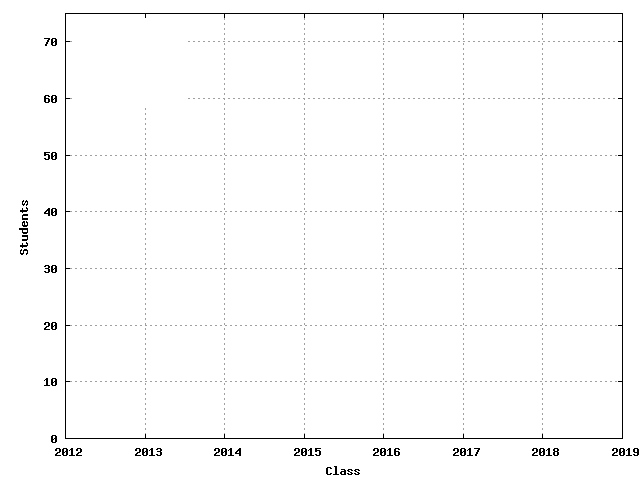
\includegraphics[scale=0.5]{ethnic.png}
\caption{CSE Student Ethnicity per Year}
\label{fig:ethnic}
\end{figure}


\end{document}

